\documentclass[11pt,letterpaper,numbers=noenddot]{scrartcl}
\usepackage[T1]{fontenc}
\usepackage[utf8]{inputenc}
\usepackage[margin=1.15in]{geometry}
\IfFileExists{newpxtext.sty}{\usepackage{newpxtext,newpxmath}}{\usepackage{mathpazo}}
\usepackage{amsmath,amssymb,amsthm,mathtools}
\usepackage{microtype,booktabs,array,enumitem,needspace}
\usepackage{xcolor,tikz}
\usetikzlibrary{arrows.meta,positioning,calc}
\usepackage[colorlinks=true,linkcolor=MidnightBlue,citecolor=MidnightBlue,urlcolor=MidnightBlue]{hyperref}
\definecolor{MidnightBlue}{RGB}{28,57,79}
\definecolor{PaleBlue}{RGB}{238,244,248}
\setkomafont{title}{\normalfont\LARGE\bfseries}
\setkomafont{author}{\normalfont\normalsize}
\setkomafont{date}{\normalfont\normalsize}
\setkomafont{section}{\normalfont\large\bfseries}
\setkomafont{subsection}{\normalfont\normalsize\bfseries}
\RedeclareSectionCommand[beforeskip=1.7ex plus .7ex minus .2ex,afterskip=.7ex plus .2ex]{section}
\RedeclareSectionCommand[beforeskip=1.4ex plus .6ex minus .2ex,afterskip=.5ex plus .2ex]{subsection}
\setlength{\parindent}{0pt}
\setlength{\parskip}{.35em}
\setlength{\emergencystretch}{2em}
\linespread{1.04}
\widowpenalty=10000
\clubpenalty=10000
\displaywidowpenalty=10000
\renewcommand{\topfraction}{.95}
\renewcommand{\textfraction}{.05}
\renewcommand{\floatpagefraction}{.85}
\setlist{nosep,leftmargin=1.5em}
\numberwithin{equation}{section}
\newtheorem{theorem}{Theorem}[section]
\newtheorem{proposition}[theorem]{Proposition}
\newtheorem{lemma}[theorem]{Lemma}
\newtheorem{corollary}[theorem]{Corollary}
\theoremstyle{definition}
\newtheorem{definition}[theorem]{Definition}
\newcommand{\Rigid}{\operatorname{Rigid}}
\newcommand{\RigidStr}{\operatorname{RigidStr}}
\newcommand{\ND}{\operatorname{ND}}
\newcommand{\Rep}{\operatorname{RepPower}_1}
\newcommand{\RepK}{\operatorname{RepPower}}
\newcommand{\Peano}{\operatorname{Peano}}
\newcommand{\Pow}{\operatorname{Pow}}
\newcommand{\Arith}{\operatorname{Arith}}
\newcommand{\Real}{\operatorname{Real}}
\newcommand{\CH}{\operatorname{CH}}
\newcommand{\PP}{\mathsf P}
\newcommand{\FTN}{\mathrm{FTN}}
\newcommand{\SOAN}{\mathrm{SOAN}}
\newcommand{\ANA}{\mathrm{ANA}}
\newcommand{\ArN}{\mathrm{ArN}}
\newcommand{\NAr}{\mathrm{NAr}}
\newcommand{\NAn}{\mathrm{NAn}}
\newcommand{\Ntwo}{\mathrm{N2An}}
\newcommand{\NCCH}{\mathrm{NCCH}}
\newcommand{\Ns}{\mathbb N}
\newcommand{\restr}{\mathbin{\upharpoonright}}
\hypersetup{pdftitle={Finite-Type Necessitism},pdfauthor={Daniel Kodsi, with assistance from GPT-6 Astra (OpenAI)},pdfsubject={Finite arithmetic hierarchies and the entailment structure of mathematical non-contingency}}
\title{Finite-Type Necessitism}
\subtitle{Arithmetic, analysis, and mathematical non-contingency}
\author{Daniel Kodsi\\\small With assistance from GPT-6 Astra (OpenAI)}
\date{30 October 2026}

\begin{document}
\maketitle
\begin{abstract}
Finite-Type Necessitism requires every possibly realizable finite arithmetic hierarchy to have a rigid realization at the same carrier type, with a full rigid represented power of its last stage. Over Classicism, its height-zero fragment entails Arithmetic Necessitism, Necessity of Arithmetic, and Necessity of Analysis; its height-one fragment is equivalent to Second-Order Analytic Necessitism. The full schema entails all seven existing mathematical non-contingency principles considered here. A uniform family of two-point models shows that each exact-height fragment is independent of all the others, and that the existing principles do not jointly entail the full schema.
\end{abstract}

\section{The principle}

We work over Classicism $C$, with the relational simple types and conventions of the Classicism map \cite{map}. The base types are $e$ and $t$; a function type is admitted only when its codomain is not $e$. Functions between carriers are represented by relations. The modalities are native:
\[
\Box p:=(p=\top),\qquad \Diamond p:=(p\ne\bot).
\]
Type letters and finite heights index schemas, not object-language quantifiers. Quantification over a structure abbreviates quantification over a finite tuple of specified types.

\subsection{Rigidity and represented powers}

For unary properties, write
\[
Y\le X\quad\Longleftrightarrow\quad
\Box\forall x\,(Yx\to Xx).
\]
The map's rigidity predicate is
\begin{equation}\label{eq:rigidity}
\begin{split}
\Rigid(X):={}&\Box\forall x\,(Xx\to\Box Xx)\\
&{}\land\Box\forall Z\left[
  \bigl(\forall x\,(Xx\to\Box Zx)\bigr)
  \to\Box\forall x\,(Xx\to Zx)\right].
\end{split}
\end{equation}
The same definition applies to relations by using tuples of arguments. Necessary distinctness is
\[
\ND(X):=\forall x,y\in X\,(x\ne y\to\Box(x\ne y)).
\]
We use \emph{rigid structure} to mean that its carriers and relations are rigid and that the members of each carrier are necessarily distinct.

A unary represented power is given by the map's formula
\begin{equation}\label{eq:rep}
\begin{split}
\Rep(Q,X):={}&\Rigid(Q)\\
&{}\land\forall B\left[QB\to
  \left(\Rigid(B)\land\forall x\,(Bx\to Xx)\right)\right]\\
&{}\land\Box\forall F\exists B\left[
  QB\land\forall x\in X\,(Bx\leftrightarrow Fx)\right].
\end{split}
\end{equation}
The canonical representative carrier is
\begin{equation}\label{eq:canonical-power}
\PP(X):=\lambda B\,\bigl(\Rigid(B)\land B\le X\bigr).
\end{equation}
For rigid $X$ with $\ND(X)$, any represented power can be taken in this canonical form; its carrier has necessarily distinct members and rigid evaluation (Lemma~\ref{lem:rigidity}).

\subsection{Finite arithmetic hierarchies}

Let $\Peano(X,z,S)$ state the usual second-order Peano axioms: $z\in X$; $S$ is a supported total functional relation on $X$; successor is injective and never has value $z$; and induction holds over every admitted subproperty of $X$.

For $X,Y:\tau t$ and $E:\tau\tau t$, put
\begin{equation}\label{eq:pow}
\begin{split}
\Pow(X,Y,E):={}&
 \forall x,y\,(E(x,y)\to Xx\land Yy)\\
&{}\land\forall F^{\tau t}\exists!y\in Y\,
 \forall x\in X\,(E(x,y)\leftrightarrow Fx).
\end{split}
\end{equation}
Thus $Y$ gives exactly one code for each extension on $X$. Define
\begin{equation}\label{eq:arith}
\Arith_n^\tau(\mathcal A):=
\Peano(X_0,z,S)\land
\bigwedge_{i<n}\Pow(X_i,X_{i+1},E_i),
\end{equation}
where
\[
\mathcal A=(X_0,\ldots,X_n,z,S,E_0,\ldots,E_{n-1}).
\]
Every $X_i$ has type $\tau t$, $z$ has type $\tau$, and $S,E_i$ have type $\tau\tau t$. The levels may overlap: their carriers and incidence relations specify their separate roles.

\begin{definition}[Finite-Type Necessitism]\label{def:ftn}
\emph{Finite-Type Necessitism} is the following schema, for every type $\tau$ and every finite $n\ge0$:
\begin{equation}\label{eq:ftn}
\boxed{
\begin{aligned}
\Diamond\exists\mathcal A\,\Arith_n^\tau(\mathcal A)
\ \longrightarrow\
\exists\mathcal A\bigl[
 &\Arith_n^\tau(\mathcal A)\\
 &{}\land\RigidStr(\mathcal A)\\
 &{}\land\Rep(\PP(X_n),X_n)
\bigr].
\end{aligned}}
\end{equation}
Write $F_n$ for the schema obtained by fixing the height $n$ and allowing every carrier type $\tau$. Thus $\FTN=\{F_n:n\in\mathbb N\}$.
\end{definition}

The additional represented power is at the native predicate type: its members have type $\tau t$, and need not fit into $\tau$.

\section{Necessary correctness and transport}

\begin{lemma}[Rigidity facts]\label{lem:rigidity}
Rigid coextensive relations are identical. Formulas whose parameters and bound variables range over rigid carriers with necessarily distinct members, and whose atomic relations are rigid and supported there, have necessary truth or necessary falsity; the relations they define on those carriers are rigid.

For rigid $X$ with $\ND(X)$, any full rigid represented power can be replaced by $\PP(X)$. Its representative carrier has necessarily distinct members, and restricted evaluation $QB\land Xx\land Bx$ is rigid.
\end{lemma}

\begin{proof}
Necessary coextension implies identity in $C$. Formula induction uses persistence for positive atoms, necessary distinctness and inextensibility for negative atoms, and inextensibility or a persistent counterexample for universal quantifiers. The hypotheses persist: rigidity has leading boxes, necessary distinctness becomes necessary by inextensibility of the carrier's square, and boxed hypotheses persist by axiom $4$. Necessitation is applied to proved conditionals.

Every rigid subproperty of $X$ agrees with a supplied representative, hence is identical to it; necessary coextension identifies the representative carrier with $\PP(X)$. Distinct representatives differ on $X$, and persistence and inextensibility preserve that difference. Evaluation is rigid by inextensibility first for each representative and then for its carrier.
\end{proof}

\begin{lemma}[Restriction and transport]\label{lem:transport}
A full rigid represented power of a rigid carrier with necessarily distinct members restricts to every rigid subcarrier. It transports along a rigid necessary bijection, and pulls back along a rigid necessary injection.
\end{lemma}

\begin{proof}
For restriction to $X'$, replace each representative $B$ by
$\lambda x\,(X'x\land Bx)$. Each restriction is rigid by Lemma~\ref{lem:rigidity}; their carrier is a term-defined image of a rigid carrier, hence rigid. Representing a predicate after restricting it to $X'$ gives necessary fullness.

For transport along a bijection $J:X\to Y$, push $B$ forward to
\[
\lambda y\,\bigl(Yy\land\exists x\in X\,(J(x,y)\land Bx)\bigr).
\]
Each pushforward and their carrier are rigid; pulling predicates back proves necessary fullness. An injection factors through its rigid image. Necessary distinctness passes to subcarriers and across necessary bijections.
\end{proof}

\begin{lemma}[Necessary correctness]\label{lem:necessary}
For every $n$ and $\tau$, $C$ proves
\begin{equation}\label{eq:necessary}
\begin{split}
\Arith_n^\tau(\mathcal A)\land\RigidStr(\mathcal A)
\land\Rep(\PP(X_n),X_n)
\ \longrightarrow\
\Box\Arith_n^\tau(\mathcal A).
\end{split}
\end{equation}
\end{lemma}

\begin{proof}
Support of a rigid relation on persistent carriers becomes necessary by the relation's inextensibility. This handles the support axioms for $S$ and the $E_i$. Each coded power supplies a singleton-code injection $X_i\to X_{i+1}$. Its graph is
\[
X_i x\land X_{i+1}y\land
\forall u\in X_i\,(E_i(u,y)\leftrightarrow u=x).
\]
Lemma~\ref{lem:rigidity} makes this graph rigid and its totality, functionality and injectivity necessary. Composition embeds every $X_i$ rigidly and necessarily into $X_n$.

Pull the top represented power back to each $X_i$ by Lemma~\ref{lem:transport}. Necessary fullness allows the predicate quantifiers in induction and power-fullness to be replaced by quantifiers over these rigid representative carriers. Lemma~\ref{lem:rigidity} then makes every hierarchy axiom necessary.
\end{proof}

\begin{lemma}[Peano matching]\label{lem:peano-match}
Given two necessarily Peano presentations with persistent successor relations, if one number carrier is rigid and has necessarily distinct members, so does the other. The two presentations are related by a rigid necessary bijection.
\end{lemma}

\begin{proof}
Define $J$ as the least relation containing the pair of zeros and closed under taking the two successors together. Second-order induction makes $J$ a bijection. The boxed Peano hypotheses make this necessary. Its least construction is persistent: $\Box J$ contains the zero pair and is successor-closed, so leastness gives $J\subseteq\Box J$.

A persistent necessarily total functional relation on a rigid domain is rigid: apply the test predicate at each member's unique image, then use the domain's inextensibility. Thus $J$ and its range are rigid. Necessary surjectivity identifies that range with the target carrier, and necessary injectivity transfers necessary distinctness.
\end{proof}

\emph{The reference argument.}
On a rigid necessarily correct reference, Lemma~\ref{lem:rigidity} fixes first-order truth. For extensional formulas, full rigid represented powers extend this to predicate quantification by replacing predicates with representatives. Whenever the presentations are categorical, isomorphism invariance transfers that truth value to every possible presentation, including at other types. If no target presentation is possible, both conditional non-contingency disjuncts hold.

\section{The arithmetic fragment}

The map's canonical numbers at a source type $\sigma$ have type
$\nu_\sigma=(\sigma t)t$. Their zero and successor are
\begin{align*}
0_\sigma&:=\lambda U^{\sigma t}\,\forall x^\sigma\,\neg Ux,\\
S_\sigma a&:=\lambda U^{\sigma t}\,\exists x^\sigma
 \bigl[Ux\land a(\lambda y^\sigma\,(Uy\land y\ne x))\bigr].
\end{align*}
Let $\Ns_\sigma$ be the least property containing $0_\sigma$ and closed under $S_\sigma$. Write
\begin{align}
I_\sigma^*&:=
 \bigl[\forall a\in\Ns_\sigma\,S_\sigma a\ne0_\sigma\bigr]
 \land
 \bigl[\forall a,b\in\Ns_\sigma\,
 (S_\sigma a=S_\sigma b\to a=b)\bigr],\label{eq:istar}\\
I_\sigma&:=\Diamond I_\sigma^*.
\end{align}
Goodsell's arithmetic interpretation lemma gives $I_\sigma\to I_\sigma^*$ in $C$ \cite[Lemma 1]{goodsell}. Induction is built into the definition of $\Ns_\sigma$.

For every finite type $\rho$, already over $C$,
\[
\Box I_\rho^*\longrightarrow\Box I_{et}^*.
\]
To see this, use the rigid finite initial segments of the necessarily Peano $\Ns_\rho$ as size standards. Failure of $I_{et}^*$ would produce a successor collision and hence a necessarily empty predicate for some positive finite cardinality, giving a necessary finite bound on $et$. The necessary injections $a\mapsto\lambda x(x=a)$ and $p\mapsto\lambda x\,p$ transfer this bound to $e$ and $t$. Counting profiles over the finitely many Boolean atoms of $t$ propagates necessary finite bounds through finite type formation, contradicting $\Box I_\rho^*$. Necessitation and 4 give the boxed conclusion. No instance of FTN is used.

The map's \emph{Arithmetic Necessitism} ($\ArN$) and \emph{Necessity of Arithmetic} ($\NAr$) are respectively
\begin{align}
\ArN:\quad&\Box I_\sigma^*\to
 [\Rigid(\Ns_\sigma)\land\ND(\Ns_\sigma)],\label{eq:arn}\\
\NAr:\quad&\Box(I_\sigma\to A)\lor
 \Box(I_\sigma\to\neg A),\label{eq:nar}
\end{align}
where $A$ ranges over first-order arithmetical sentences at $\sigma$ \cite{map,bg}.

\begin{theorem}\label{thm:f0-arith}
Over $C$, $F_0$ entails both Arithmetic Necessitism and Necessity of Arithmetic.
\end{theorem}

\begin{proof}
Assume $\Box I_\sigma^*$. The canonical numbers form a Peano presentation at $\nu_\sigma$, activating $F_0$ there. Lemmas~\ref{lem:necessary} and~\ref{lem:peano-match} make the resulting rigid reference necessarily Peano and transfer its rigidity and necessary distinctness to $\Ns_\sigma$, proving \eqref{eq:arn}. Canonical numberhood is persistent by its least-inductive construction; the closed successor term's graph is persistent by necessity of identity, as matching requires.

For \eqref{eq:nar}, $I_\sigma$ similarly activates $F_0$. Arithmetic recursion gives rigid addition and multiplication on its reference. Goodsell's lemma makes the canonical numbers Peano wherever $I_\sigma$ holds, so Peano categoricity and the reference argument fix their arithmetical truth. If $\neg I_\sigma$, S4 gives $\Box\neg I_\sigma$, making both disjuncts true.
\end{proof}

\section{Analysis and the height-one equivalence}

A real structure $\mathfrak R$ at $\tau$ consists of a carrier $X^{\tau t}$, relational order and field operations, distinguished zero and one, and its least inductive natural-number predicate. The formula $\Real_\tau(\mathfrak R)$ says that it is a complete ordered field: every admitted nonempty bounded subproperty of $X$ has a least upper bound. All analytical formulas are interpreted in this structure \cite{map,bg,bacon}.

Analytic Necessitism is the schema
\begin{equation}\label{eq:ana}
\Diamond\exists\mathfrak R\,\Real_\tau(\mathfrak R)
\to
\exists\mathfrak R\,
 [\RigidStr(\mathfrak R)\land\Box\Real_\tau(\mathfrak R)].
\end{equation}
Second-Order Analytic Necessitism adds full rigid represented powers of every finite relation arity. For each $m\ge1$, its consequent requires
\begin{equation}\label{eq:soan-old}
\exists\mathfrak R\,Q_1\cdots Q_m\,
 \left[\RigidStr(\mathfrak R)\land\Box\Real_\tau(\mathfrak R)
 \land\bigwedge_{k=1}^m\RepK_k(Q_k,X)\right].
\end{equation}

\begin{lemma}[Unary form of SOAN]\label{lem:soan-unary}
SOAN is equivalent over $C$ to
\begin{equation}\label{eq:soan}
\begin{split}
\Diamond\exists\mathfrak R\,\Real_\tau(\mathfrak R)
\to\exists\mathfrak R\,[
\Real_\tau(\mathfrak R)\land\RigidStr(\mathfrak R)
\land\Rep(\PP(X),X)].
\end{split}
\end{equation}
\end{lemma}

\begin{proof}
Replacing predicates by unary representatives makes completeness and leastness of the number predicate necessary; the field axioms are already stable by Lemma~\ref{lem:rigidity}. Thus the consequent implies $\Box\Real_\tau(\mathfrak R)$.

Finite tuples inject definably into the reals: code each real by its rational cut, interleave the resulting subsets of the numbers, and use a Cantor-set code. On a rigid necessarily real structure these injections are rigid, so pulling back unary representatives supplies full represented powers of every finite arity. Conversely, take the unary power in \eqref{eq:soan-old} and normalize its carrier by Lemma~\ref{lem:rigidity}.
\end{proof}

\Needspace{8\baselineskip}
\begin{lemma}[Numbers, subsets, and reals]\label{lem:codes}
For each $\tau$, $C$ proves
\begin{equation}\label{eq:exist-equiv}
\exists\mathcal A\,\Arith_1^\tau(\mathcal A)
\quad\longleftrightarrow\quad
\exists\mathfrak R\,\Real_\tau(\mathfrak R).
\end{equation}
\end{lemma}

\begin{proof}
Given a Peano carrier $N$ and its full extensional subset-code carrier $C$, code the rationals in $N$ by reduced fractions. The elements of $C$ whose rows are rational Dedekind cuts form a carrier $X\subseteq C$. Their field operations are specified by the ordinary cut constructions. For any admitted nonempty bounded family $Y$ of cuts, the predicate
\[
q\longmapsto\exists c\in X\,(Yc\land E(q,c))
\]
is an admitted subproperty of $N$. Its unique code in $C$ gives the union cut and hence the least upper bound. The natural-number predicate is the range of the rational-cut embedding of $N$, and induction proves its leastness. This gives a real structure at $\tau$.

Conversely, use a real field's number predicate and code a subproperty $B$ of those numbers by
\[
\sup_m\sum_{k<m}\frac{\chi_B(k)}{4^{k+1}}.
\]
The sums and their codes are defined by Peano recursion; completeness supplies the supremum. At the first differing digit, its contribution exceeds the entire possible tail. Thus codes agree exactly when the predicates agree on the numbers. The codes and their digit-incidence relation give a full extensional power presentation, with both carriers at $\tau$. These are relational definitions and require no Choice principle.
\end{proof}

\begin{theorem}[Height one]\label{thm:height-one}
At each carrier type, height-one FTN is equivalent to SOAN; hence
\begin{equation}\label{eq:f1}
\boxed{F_1\longleftrightarrow\SOAN.}
\end{equation}
\end{theorem}

\begin{proof}
Lemma~\ref{lem:codes} identifies the possibility antecedents. From a height-one FTN witness, Lemma~\ref{lem:necessary} gives a necessarily correct rigid presentation of numbers and their subsets. Its Dedekind-cut field is a rigid subcarrier of the subset-code carrier $C$. Restrict the supplied represented power of $C$ to this field. Lemma~\ref{lem:soan-unary} gives SOAN.

Conversely, let SOAN supply a rigid necessarily real field $X$ and its full rigid represented unary power. Restrict that power to its rigid number carrier $N$, obtaining a rigid representative carrier $Q_N$. Define the Cantor-code map on $Q_N\times X$. Its graph is given by its finite prefix sums and bounds, a formula over these rigid carriers and $N$, so is rigid and necessarily total and injective. Its image $C$ is rigid, and its digit-incidence relation is rigid. Necessary fullness of $Q_N$ makes $(N,C)$ a necessarily full extensional presentation. Restrict the represented power of $X$ to $C$. These witnesses satisfy the height-one FTN consequent.
\end{proof}

\subsection{The analytical truth principles}

For an analytical sentence $A$, the map's non-contingency assertion is
\begin{equation}\label{eq:analytic-truth}
\begin{split}
&\Box\forall\mathfrak R\,
 (\Real_\tau(\mathfrak R)\to A(\mathfrak R))\\
&\qquad{}\lor
\Box\forall\mathfrak R\,
 (\Real_\tau(\mathfrak R)\to\neg A(\mathfrak R)).
\end{split}
\end{equation}
\emph{Necessity of Analysis} ($\NAn$) restricts $A$ to first-order analytical sentences; \emph{Necessity of Second-Order Analysis} ($\Ntwo$) permits all finite relation arities. The outer disjunction fixes one truth value across all possible presentations.

\begin{theorem}\label{thm:analysis}
Over $C$,
\[
F_0\Rightarrow\NAn,\qquad
\ANA\Rightarrow\NAn,\qquad
\SOAN\Rightarrow\Ntwo.
\]
\end{theorem}

\begin{proof}
Suppose a real structure is possible at $\tau$. Its number substructure activates $F_0$ there, supplying a rigid necessarily Peano carrier and its full rigid first power. The cut construction of Lemma~\ref{lem:codes}, with the native power as subset-code carrier, gives a rigid necessarily real field at $\tau t$. Completeness needs only unions of cuts, represented as predicates on the number carrier. Cross-type categoricity of complete ordered fields \cite[Appendix C]{bacon} and the reference argument now give $\NAn$. ANA supplies the real reference directly.

SOAN supplies full represented powers for the finitely many relation arities occurring in each second-order sentence. Since analytical formulas depend only on relation extensions, replacing predicates by representatives preserves truth necessarily. Pullback and pushforward along the categorical field isomorphism give second-order invariance, so the same reference argument yields $\Ntwo$.
\end{proof}

In the map's formulation, the continuum hypothesis is
\begin{equation}\label{eq:ch}
\CH(\mathfrak R):=
\forall Y\subseteq X\,
 (Y\precsim N\lor Y\approx X),
\end{equation}
where $\precsim$ and $\approx$ mean relational injection and bijection: every subcollection is at most countable or equinumerous with the reals. This is second-order analytical, and $\NCCH$ is \eqref{eq:analytic-truth} with $A=\CH$.

\begin{corollary}\label{cor:all}
FTN entails all seven principles listed in Figure~\ref{fig:entailments}, without any additional existence assumption.
\end{corollary}

\section{The entailment structure}

Figure~\ref{fig:entailments} records the proved entailments; omitted arrows are not asserted non-entailments. The preceding results give the arrows, with $\Ntwo\Rightarrow\NAn$ and $\Ntwo\Rightarrow\NCCH$ by restriction. Section~\ref{sec:lattice} establishes the fragment separations.

\begin{figure}[htbp]
\centering
\begin{minipage}[c]{.64\linewidth}
\centering
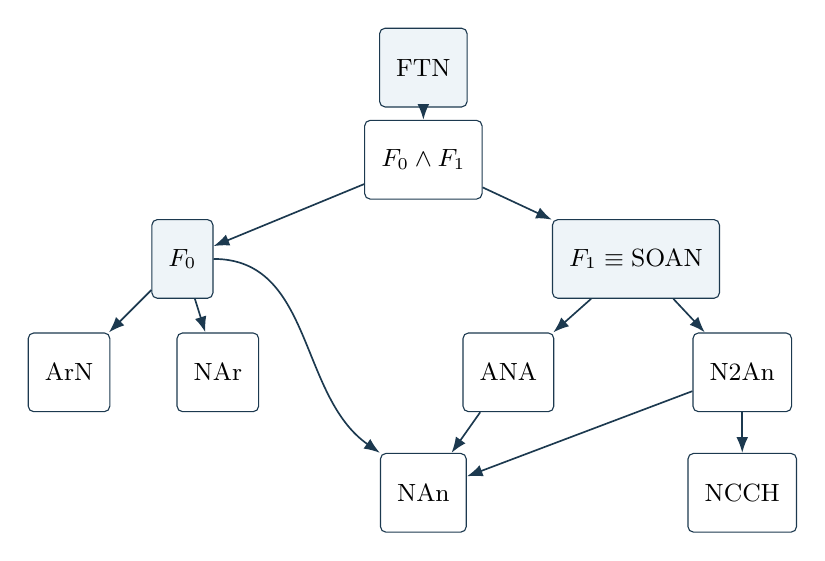
\begin{tikzpicture}[
  x=.9cm,y=.9cm,
  >=Latex,
  node distance=10mm,
  every node/.style={font=\small},
  principle/.style={draw=MidnightBlue,rounded corners=2pt,align=center,inner sep=6pt,minimum height=10mm},
  major/.style={principle,fill=PaleBlue},
  arrow/.style={->,draw=MidnightBlue,semithick}
]
\node[major] (ftn) at (0,4.8) {$\FTN$};
\node[principle] (both) at (0,3.5) {$F_0\land F_1$};
\node[major] (f0) at (-3.4,2.1) {$F_0$};
\node[major] (f1) at (3.0,2.1) {$F_1\equiv\SOAN$};
\node[principle] (arn) at (-5.0,.5) {$\ArN$};
\node[principle] (nar) at (-2.9,.5) {$\NAr$};
\node[principle] (ana) at (1.2,.5) {$\ANA$};
\node[principle] (n2) at (4.5,.5) {$\Ntwo$};
\node[principle] (nan) at (0,-1.2) {$\NAn$};
\node[principle] (ch) at (4.5,-1.2) {$\NCCH$};
\draw[arrow] (ftn)--(both);
\draw[arrow] (both)--(f0);
\draw[arrow] (both)--(f1);
\draw[arrow] (f0)--(arn);
\draw[arrow] (f0)--(nar);
\draw[arrow] (f0.east) to[out=0,in=145] (nan.north west);
\draw[arrow] (f1)--(ana);
\draw[arrow] (f1)--(n2);
\draw[arrow] (ana)--(nan);
\draw[arrow] (n2)--(nan);
\draw[arrow] (n2)--(ch);
\end{tikzpicture}
\end{minipage}\hfill
\begin{minipage}[c]{.33\linewidth}
\small
\begin{tabular}{@{}l>{\raggedright\arraybackslash}p{.70\linewidth}@{}}
\toprule
$\ArN$ & Arithmetic Necessitism\\
$\NAr$ & Necessity of Arithmetic\\
$\ANA$ & Analytic Necessitism\\
$\SOAN$ & Second-Order Analytic Necessitism\\
$\NAn$ & Necessity of Analysis\\
$\Ntwo$ & Necessity of Second-Order Analysis\\
$\NCCH$ & Non-contingency of the Continuum Hypothesis\\
\bottomrule
\end{tabular}
\end{minipage}
\caption{Arrows run from stronger to weaker principles. Intermediate cumulative fragments between FTN and $F_0\land F_1$ are omitted.}
\label{fig:entailments}
\end{figure}

For a first-order sentence $\varphi$ in a finite hierarchy's many-sorted arithmetic-and-membership signature, with sort-respecting equality and quantifiers restricted to its displayed levels, FTN entails
\begin{equation}\label{eq:finite-truth}
\begin{split}
&\Box\forall\mathcal A\,
 (\Arith_n^\tau(\mathcal A)\to\varphi(\mathcal A))\\
&\qquad{}\lor
\Box\forall\mathcal A\,
 (\Arith_n^\tau(\mathcal A)\to\neg\varphi(\mathcal A)).
\end{split}
\end{equation}
Here $F_n$ supplies the reference, and Peano matching followed by membership-row matching gives categoricity. The reference argument proves \eqref{eq:finite-truth}.

FTN also extends a realized hierarchy through any finite number of native powers. If levels occupy different types, singleton codes embed each finite prefix into its last carrier's type. Apply the corresponding $F_i$, then match number bases and membership rows to assemble rigid witnesses at the original types. The extra native power adds a level; repeat finitely. This provides sufficiently long rigid full presentations for ordinary extensional finite-type mathematics. Higher predicates must respect agreement of lower-type arguments. The reference argument fixes each sentence's truth value without deciding which it has.

\section{Strictness and the finite-height lattice}\label{sec:lattice}

The finite heights impose independent realization requirements. We establish this with one family of full two-point models.

\subsection{The full two-point model}

Work in an ordinary set-theoretic metatheory with Choice. Take nonempty sets $A\subseteq B$ and two points $r\to s$, with reflexive accessibility. At $s$ use the full extensional type hierarchy over $D_e^s=B$, with $D_t^s=2$. At $r$, put $D_e^r=A$ and let $\pi_e:A\hookrightarrow B$ be inclusion.

Every relational type has a flattened presentation $\tau=\sigma_1\cdots\sigma_k t$. Define recursively
\begin{equation}\label{eq:profiles}
D_\tau^r=
2^{\prod_iD_{\sigma_i}^r}\times D_\tau^s,
\qquad
\pi_\tau(F_0,F_1)=F_1.
\end{equation}
In particular, $D_t^r=2\times2$. A relation object specifies its extensions at both points. Application uses $F_0$ at root arguments and $F_1$ at their projections. Connectives act coordinatewise, while equality and quantification are
\begin{align}
\operatorname{Eq}_r(x,y)
 &=\bigl(\delta[x=y],\delta[\pi x=\pi y]\bigr),\label{eq:model-eq}\\
\forall_r(F_0,F_1)
 &=\left(\bigwedge_{x\in D_\sigma^r}F_0(x),
          \bigwedge_{b\in D_\sigma^s}F_1(b)\right).
\end{align}
Lambda abstraction is interpreted by its two profiles. Projection commutes with application and logical operations. The higher-order logical axioms hold at each coordinate, and H-equivalent lambda bodies have equal profiles at both coordinates, validating the Logical Equivalence schema of $C$. This is the full action construction for a single arrow. Native necessity and possibility are
\[
\Box(b,a)=(b\land a,a),\qquad
\Diamond(b,a)=(b\lor a,a).
\]

For a relation with extensions $E_r,E_s$, the definitions give
\begin{equation}\label{eq:model-rigid}
\Rigid(E)\text{ at }r\quad\Longleftrightarrow\quad
E_s=\pi[E_r].
\end{equation}
Persistence gives one inclusion. For the other, use the admitted test relation with extensions $E_r$ and $\pi[E_r]$ in the inextensibility condition. Necessary distinctness of a carrier is exactly injectivity of $\pi$ on its root extension.

Consequently, a carrier on which projection is bijective supports a rigid structure whenever the structures at the two points correspond. It has a full rigid represented native power: the representatives are precisely the paired characteristic predicates of $U\subseteq E_r$ and $\pi[U]\subseteq E_s$. All such predicates are admitted by \eqref{eq:profiles}.

\subsection{A separate requirement at every height}

Let $\beth_0=\aleph_0$ and $\beth_{n+1}=2^{\beth_n}$. Full predicate extensions at each point ensure that a Peano carrier has size $\beth_0$ and that the successive code carriers in $\Arith_n$ have sizes $\beth_1,\ldots,\beth_n$. Since levels may overlap, a type can realize $\Arith_n$ exactly when its domain has at least $\beth_n$ members.

\begin{theorem}[Exact-height independence]\label{thm:independence}
For every finite $j\ge0$, there is a model of $C$ satisfying every $F_n$ with $n\ne j$ and falsifying $F_j$.
\end{theorem}

\begin{proof}
Use the two-point construction with
\begin{equation}\label{eq:cardinal-models}
(|A|,|B|)=
\begin{cases}
(1,\beth_0),&j=0,\\
(\beth_{j-1},\beth_j),&j\ge1.
\end{cases}
\end{equation}
At individual type, an $n$-height presentation is possible exactly when $n\le j$. For $n<j$, choose the whole finite hierarchy inside $A$ and transport it by inclusion. Projection is bijective on every chosen carrier, so the hierarchy and its full native top power satisfy the $F_n$ consequent. For $n=j$, the presentation exists at $s$ but cannot exist at $r$, whose individual domain is too small. For $n>j$, the antecedent is false at both points.

It remains to check every relational type. Structural induction in \eqref{eq:profiles} shows that a type with finite terminal domain also has finite root domain, while each relational type with infinite terminal domain has
\[
|D_\tau^r|=|D_\tau^s|.
\]
For the infinite case, the root profile factor has size at most the terminal function domain: finite argument factors do not change the relevant infinite cardinal products. The terminal factor gives the opposite inequality. Moreover, projection at every relational type has the explicit section $a\mapsto(0,a)$.

Thus any possible finite arithmetic hierarchy at a relational type can be selected terminally and lifted along that section. The lifted carriers project bijectively, their relations can be specified by paired profiles, and their full rigid native top power is supplied as above. If a hierarchy is first witnessed at $r$, equality of the infinite domain cardinalities ensures a terminal realization of the same height. Finite domains admit no Peano presentation. Hence every relational-type instance holds, and the only failing height is $j$, at $e$.
\end{proof}

\begin{corollary}[The finite-height lattice]\label{cor:order}\label{cor:strict-old}
For any set $S$ of finite heights and any finite $m$,
\begin{equation}\label{eq:order}
C+\{F_n:n\in S\}\vdash F_m
\quad\Longleftrightarrow\quad m\in S.
\end{equation}
Thus entailment among conjunctions of exact-height schemas is reverse inclusion of the required heights. The cumulative fragments $G_n:=F_0\land\cdots\land F_n$ form the strict chain
\begin{equation}\label{eq:strict-chain}
\FTN\ \Longrightarrow\ \cdots\ \Longrightarrow\ G_2
\ \Longrightarrow\ G_1
\ \Longrightarrow\ G_0,
\end{equation}
with
\[
G_0=F_0,\qquad G_1=F_0\land\SOAN.
\]
No finite collection of heights entails FTN. Moreover, $F_0$ and SOAN are incomparable, $F_0\not\Rightarrow\ANA$, and the seven existing principles in Corollary~\ref{cor:all} do not jointly entail FTN.
\end{corollary}

\begin{proof}
If $m\notin S$, the $j=m$ model of Theorem~\ref{thm:independence} witnesses failure of entailment; if $m\in S$, entailment is immediate. This proves \eqref{eq:order} and the chain's strictness.

The $j=0,1$ models separate $F_0$ and SOAN. For $j=1$, a real field on individuals is possible at $s$, while the countable root domain with full predicate extensions admits no complete real field. Hence $F_0\not\Rightarrow\ANA$.

For $j=2$, the individual domains have sizes $\beth_1$ and $\beth_2$. The model satisfies $F_0\land F_1$, hence all seven existing principles, but fails $F_2$. A rigid continuum and all its native represented powers are available, while a height-two arithmetic hierarchy fits into the individual domain only at the second point.
\end{proof}

Full FTN is consistent: every one-point full extensional type model satisfies it, since all relations are rigid and native powers are full.

\clearpage
\appendix
\section{Invariance}\label{sec:invariance}

Define \emph{invariance} by
\begin{equation}\label{eq:invariance}
\operatorname{Invariant}(X):=
\Box\forall x\,(\Diamond Xx\to\Box Xx).
\end{equation}
Since $(\Diamond A\to\Box A)\leftrightarrow(\Box A\lor\Box\neg A)$, invariance is persistence of both $X$ and its pointwise complement. Replacing persistence by invariance in rigidity gives
\begin{equation}\label{eq:invariant-rigidity}
\begin{split}
\Rigid^\diamond(X)
&:=\operatorname{Invariant}(X)\land\operatorname{Inextensible}(X)\\
&\longleftrightarrow
\Rigid(X)\land\operatorname{Persistent}(\neg X),
\end{split}
\end{equation}
where inextensibility is the second conjunct of \eqref{eq:rigidity}.

Write $\mathsf 5:=\forall p\,(\Diamond\Box p\to\Box p)$; adding $\Box\mathsf 5$ to $C$ gives the map's $C5$ background. The singleton $T:=\lambda p\,(p=\top)$ is rigid and has necessarily distinct members in $C$, whereas
\begin{equation}\label{eq:invariant-singleton}
\Rigid^\diamond(T)\longleftrightarrow\Box\mathsf 5.
\end{equation}
Its invariance clause is $\Box\forall p\,(\Diamond\Box p\to\Box\Box p)$, equivalent to $\Box\mathsf 5$ by T and 4. Ordinary rigidity thus permits something outside a carrier to become identical to a member; invariance excludes this.

Let $\FTN^\diamond$ denote the variant obtained by substituting $\Rigid^\diamond$ throughout FTN, including in represented powers and $\PP(X)$.

\begin{theorem}\label{thm:invariant-ftn}
Over $C$, $\FTN^\diamond$ is equivalent to FTN together with the schema
\begin{equation}\label{eq:invariant-ftn-guard}
\Diamond\exists\mathcal A\,\Arith_0^\tau(\mathcal A)
\longrightarrow\Box\mathsf 5.
\end{equation}
Hence, whenever a Peano presentation is possible at some type,
$\FTN^\diamond$ is equivalent to $\FTN+\Box\mathsf 5$.
\end{theorem}

\begin{proof}
A modified represented power has an invariant, inextensible representative carrier $Q$ whose members are themselves invariant and inextensible. Distinct members differ at an argument by Lemma~\ref{lem:rigidity}; invariance preserves that difference, so $Q$ has necessarily distinct members. For $QB$,
\[
\forall D\,\bigl(\Diamond(D=B)\to D=B\bigr):
\]
possible identity gives possible membership in $Q$, hence membership by invariance, after which necessary distinctness gives identity.

Fullness supplies a member $B\in Q$. On the inhabited argument type of an FTN witness, put $D_p:=\lambda x\,(p\leftrightarrow Bx)$. Boolean cancellation gives
$D_p=B\leftrightarrow p=\top\leftrightarrow\Box p$.
The preceding implication yields $\mathsf 5$. The argument also holds necessarily: $\Rigid^\diamond$ has leading boxes, inextensibility of $Q$ makes the condition on its members necessary, and the selected member persists. Thus every activated FTN instance supplies $\Box\mathsf 5$.

Conversely, under $\Box\mathsf 5$, ordinary persistence implies invariance: $\Diamond Xx$ gives $\Diamond\Box Xx$, hence $\Box Xx$. The rigidity definitions and their represented powers therefore coincide. Since every higher-height antecedent implies the height-zero antecedent by truncation, \eqref{eq:invariant-ftn-guard} converts every ordinary FTN witness into a modified one. The same equivalence converts the modified witnesses back.
\end{proof}

All positive consequences of FTN carry over. The strengthening is strict: the full two-point construction with $A=B=\omega$ satisfies FTN, since the relevant type capacities agree, but falsifies $\Box\mathsf 5$ and hence $\FTN^\diamond$. With $A=B=\{*\}$, all finite-type domains are finite, so $\FTN^\diamond$ holds vacuously while $\Box\mathsf 5$ fails.

The variant does not force modal collapse. A full Boolean-valued type model over $2\times2$, with crisp equality and an infinite individual domain, supplies fixed classical hierarchies and full powers represented by predicates taking only $\bot$ and $\top$. It satisfies $\FTN^\diamond$, while $(1,0)$ remains a contingent proposition.

\Needspace{9\baselineskip}
\begin{thebibliography}{9}
\small
\bibitem{map}
\emph{Logical Maps: Classicism}. Background definitions and mathematical-contingency principles, comparison version \texttt{6f15ef5c}, 30 October 2026.
\href{https://github.com/zwlgzwlg/Logical-Maps/blob/6f15ef5c491fcb117d4d11d8837545a9baaa042d/logical-maps/topics/classicism/background.md}{Background and conventions};
\href{https://github.com/zwlgzwlg/Logical-Maps/tree/6f15ef5c491fcb117d4d11d8837545a9baaa042d/logical-maps/topics/classicism/principles}{principle statements}.

\bibitem{goodsell}
Zachary Goodsell. \emph{Arithmetic is Necessary}. Draft dated 5 June 2024. Lemma 1 and the canonical arithmetic interpretation.
\href{https://philarchive.org/archive/GOOAIN}{Manuscript}.

\bibitem{bg}
Neil Barton and Zachary Goodsell. \emph{Continuum Contingency}. Draft dated 14 October 2026, especially \S\S5.7--5.9. Definitions of arithmetic and analytic necessity and necessitism.

\bibitem{bacon}
Andrew Bacon. \emph{Could the truths of mathematics have been different?} Draft dated 9 October 2025, with online appendix, especially Appendix C. Categoricity and analytical invariance.
\href{https://andrew-bacon.github.io/papers/Could\%20mathematics\%20have\%20been\%20different.pdf}{Manuscript}.
\end{thebibliography}
\end{document}
